\documentclass{article}\usepackage[]{graphicx}\usepackage[]{color}
%% maxwidth is the original width if it is less than linewidth
%% otherwise use linewidth (to make sure the graphics do not exceed the margin)
\makeatletter
\def\maxwidth{ %
  \ifdim\Gin@nat@width>\linewidth
    \linewidth
  \else
    \Gin@nat@width
  \fi
}
\makeatother

\definecolor{fgcolor}{rgb}{0.345, 0.345, 0.345}
\newcommand{\hlnum}[1]{\textcolor[rgb]{0.686,0.059,0.569}{#1}}%
\newcommand{\hlstr}[1]{\textcolor[rgb]{0.192,0.494,0.8}{#1}}%
\newcommand{\hlcom}[1]{\textcolor[rgb]{0.678,0.584,0.686}{\textit{#1}}}%
\newcommand{\hlopt}[1]{\textcolor[rgb]{0,0,0}{#1}}%
\newcommand{\hlstd}[1]{\textcolor[rgb]{0.345,0.345,0.345}{#1}}%
\newcommand{\hlkwa}[1]{\textcolor[rgb]{0.161,0.373,0.58}{\textbf{#1}}}%
\newcommand{\hlkwb}[1]{\textcolor[rgb]{0.69,0.353,0.396}{#1}}%
\newcommand{\hlkwc}[1]{\textcolor[rgb]{0.333,0.667,0.333}{#1}}%
\newcommand{\hlkwd}[1]{\textcolor[rgb]{0.737,0.353,0.396}{\textbf{#1}}}%
\let\hlipl\hlkwb

\usepackage{framed}
\makeatletter
\newenvironment{kframe}{%
 \def\at@end@of@kframe{}%
 \ifinner\ifhmode%
  \def\at@end@of@kframe{\end{minipage}}%
  \begin{minipage}{\columnwidth}%
 \fi\fi%
 \def\FrameCommand##1{\hskip\@totalleftmargin \hskip-\fboxsep
 \colorbox{shadecolor}{##1}\hskip-\fboxsep
     % There is no \\@totalrightmargin, so:
     \hskip-\linewidth \hskip-\@totalleftmargin \hskip\columnwidth}%
 \MakeFramed {\advance\hsize-\width
   \@totalleftmargin\z@ \linewidth\hsize
   \@setminipage}}%
 {\par\unskip\endMakeFramed%
 \at@end@of@kframe}
\makeatother

\definecolor{shadecolor}{rgb}{.97, .97, .97}
\definecolor{messagecolor}{rgb}{0, 0, 0}
\definecolor{warningcolor}{rgb}{1, 0, 1}
\definecolor{errorcolor}{rgb}{1, 0, 0}
\newenvironment{knitrout}{}{} % an empty environment to be redefined in TeX

\usepackage{alltt}
\usepackage[letterpaper, portrait, margin=1in]{geometry}
\usepackage{amsmath}
\IfFileExists{upquote.sty}{\usepackage{upquote}}{}
\begin{document}
\title{Problem Set 7}
\author{Jeffrey Kwarsick}

\section{Problem 1}
\subsection{Part (a)}
The pareto distribution decays more quickly than the exponential distribution.  This is illustrated below with a sample plot.  The black line is the pareto distribution and green line is the exponential distribution.
\begin{knitrout}
\definecolor{shadecolor}{rgb}{0.969, 0.969, 0.969}\color{fgcolor}\begin{kframe}
\begin{alltt}
\hlcom{################}
\hlcom{### Part (a) ###}
\hlcom{################}

\hlcom{#pareto pdf}
\hlstd{pareto} \hlkwb{<-} \hlkwa{function}\hlstd{(}\hlkwc{x}\hlstd{,} \hlkwc{alpha}\hlstd{,} \hlkwc{beta}\hlstd{) \{}
  \hlkwd{return}\hlstd{( (beta}\hlopt{*}\hlstd{alpha}\hlopt{^}\hlstd{beta)}\hlopt{/}\hlstd{(x}\hlopt{^}\hlstd{(beta}\hlopt{+}\hlnum{1}\hlstd{)) )}
\hlstd{\}}

\hlcom{#shifted exponential pdf}
\hlstd{exp.shft} \hlkwb{<-} \hlkwa{function}\hlstd{(}\hlkwc{x}\hlstd{,} \hlkwc{lambda}\hlstd{,} \hlkwc{shft}\hlstd{) \{}
  \hlkwd{return}\hlstd{( lambda}\hlopt{*}\hlkwd{exp}\hlstd{(}\hlopt{-}\hlstd{lambda}\hlopt{*}\hlstd{(x}\hlopt{-}\hlstd{shft)) )}
\hlstd{\}}

\hlcom{#pareto parameters, alpha and beta}
\hlstd{alpha}  \hlkwb{<-} \hlnum{2.0}
\hlstd{beta}   \hlkwb{<-} \hlnum{3.0}

\hlcom{#shifted exponential parameter, lambda}
\hlstd{lambda} \hlkwb{<-} \hlnum{1.0}
\hlstd{x.shft} \hlkwb{<-} \hlnum{2.0}

\hlcom{#Does the pareto decay faster or more slowly compared to exponential?}

\hlcom{#create list of x values to plug into each pdf}
\hlcom{#from 0 to 0.5, steps of 0.001}
\hlstd{x} \hlkwb{<-} \hlkwd{seq}\hlstd{(}\hlnum{0.0}\hlstd{,} \hlnum{0.5}\hlstd{,} \hlnum{0.001}\hlstd{)}

\hlcom{#plotting to show that pareto decays slower compared to exponential}
\hlkwd{plot}\hlstd{(x,} \hlkwd{pareto}\hlstd{(x,} \hlnum{0.5}\hlstd{,} \hlnum{1.0}\hlstd{),} \hlkwc{type}\hlstd{=}\hlstr{'l'}\hlstd{,}\hlkwc{ylim}\hlstd{=}\hlkwd{c}\hlstd{(}\hlnum{0}\hlstd{,}\hlnum{5}\hlstd{))}
\hlkwd{lines}\hlstd{(x,} \hlkwd{exp.shft}\hlstd{(x,} \hlnum{10}\hlstd{,} \hlnum{0}\hlstd{),} \hlkwc{col}\hlstd{=}\hlstr{'green'}\hlstd{)}
\end{alltt}
\end{kframe}
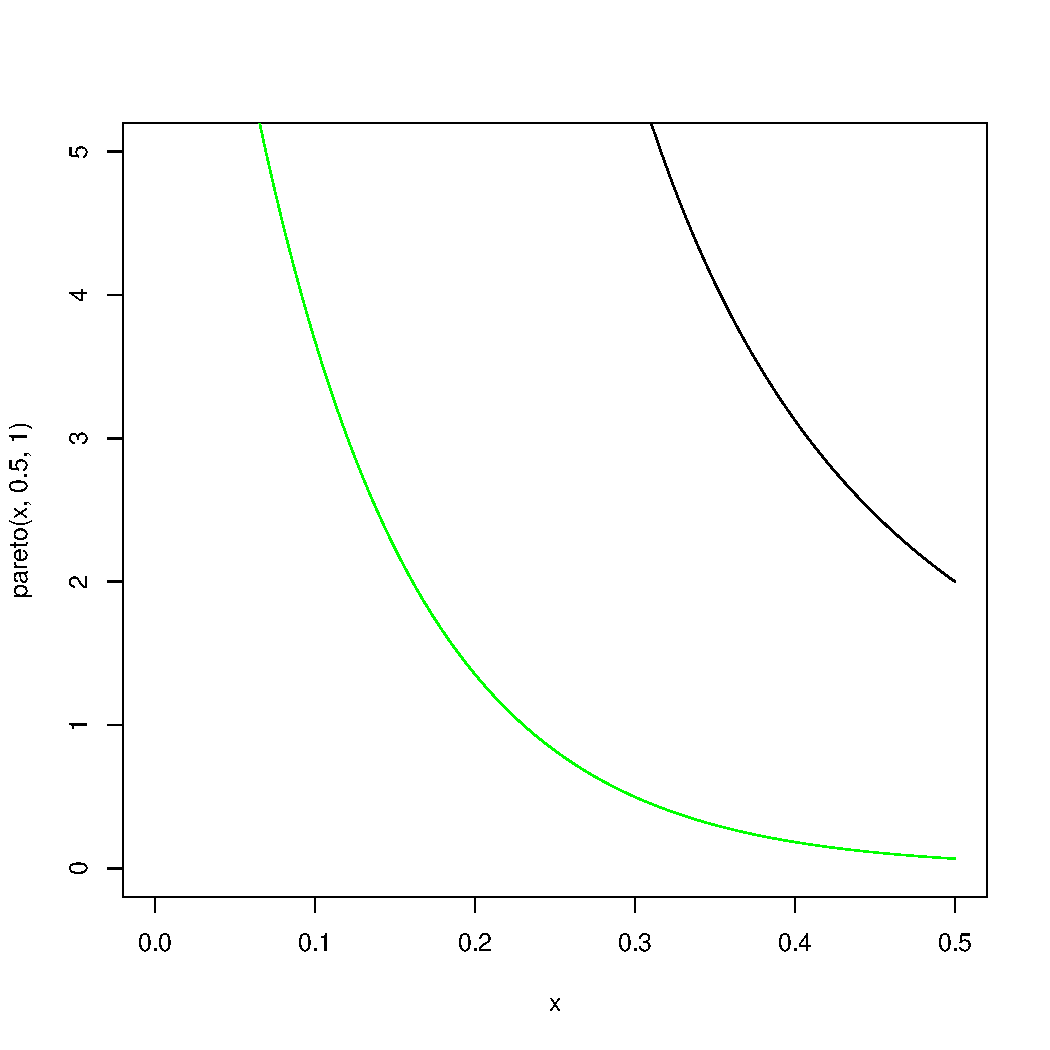
\includegraphics[width=\maxwidth]{figure/unnamed-chunk-1-1} 

\end{knitrout}
\subsection{Part (b)}
\begin{knitrout}
\definecolor{shadecolor}{rgb}{0.969, 0.969, 0.969}\color{fgcolor}\begin{kframe}
\begin{alltt}
\hlcom{################}
\hlcom{### Part (b) ###}
\hlcom{################}

\hlcom{#same seed for every iteration of running this problem}
\hlkwd{set.seed}\hlstd{(}\hlnum{1}\hlstd{)}

\hlcom{#inverse cdfs are used for inversion transformation sampling}
\hlcom{#used to sample random X_m variable}

\hlcom{#pareto pdf}
\hlstd{pareto} \hlkwb{<-} \hlkwa{function}\hlstd{(}\hlkwc{x}\hlstd{,} \hlkwc{alpha}\hlstd{,} \hlkwc{beta}\hlstd{) \{}
  \hlkwd{return}\hlstd{( (beta}\hlopt{*}\hlstd{alpha}\hlopt{^}\hlstd{beta)}\hlopt{/}\hlstd{(x}\hlopt{^}\hlstd{(beta}\hlopt{+}\hlnum{1}\hlstd{)) )}
\hlstd{\}}

\hlcom{#inverse cdf of pareto}
\hlstd{inverse.cdf.pareto} \hlkwb{<-} \hlkwa{function}\hlstd{(}\hlkwc{u}\hlstd{,} \hlkwc{alpha}\hlstd{,} \hlkwc{beta}\hlstd{) \{}
  \hlcom{#where u < 1}
  \hlkwd{return}\hlstd{( alpha}\hlopt{*}\hlstd{((}\hlnum{1} \hlopt{-} \hlstd{u)}\hlopt{^}\hlstd{(}\hlopt{-}\hlnum{1}\hlopt{/}\hlstd{beta)) )}
\hlstd{\}}

\hlcom{#shifted exponential pdf, shifted 2 units to right}
\hlstd{exp.shft} \hlkwb{<-} \hlkwa{function}\hlstd{(}\hlkwc{x}\hlstd{,} \hlkwc{lambda}\hlstd{,} \hlkwc{shft}\hlstd{) \{}
  \hlkwd{return}\hlstd{( (x} \hlopt{>=} \hlnum{2}\hlstd{)} \hlopt{*} \hlstd{lambda} \hlopt{*} \hlkwd{exp}\hlstd{(} \hlopt{-}\hlstd{lambda} \hlopt{*} \hlstd{(x} \hlopt{-} \hlstd{shft) ))}
\hlstd{\}}

\hlcom{#inverse cdf of shifted exponential}
\hlstd{inverse.cdf.exp.shft} \hlkwb{<-} \hlkwa{function}\hlstd{(}\hlkwc{u}\hlstd{) \{}
  \hlcom{#where u < 1}
  \hlcom{#lambda = 1}
  \hlkwd{return}\hlstd{(} \hlnum{2} \hlopt{-} \hlkwd{log}\hlstd{(}\hlnum{1} \hlopt{-} \hlstd{u) )}
\hlstd{\}}

\hlcom{#pareto parameters, alpha and beta}
\hlstd{alpha}  \hlkwb{<-} \hlnum{2.0}
\hlstd{beta}   \hlkwb{<-} \hlnum{3.0}

\hlcom{#shifted exponential parameter, lambda}
\hlstd{lambda} \hlkwb{<-} \hlnum{1.0}
\hlstd{x.shft} \hlkwb{<-} \hlnum{2.0}

\hlcom{#number of extimators}
\hlstd{m} \hlkwb{<-} \hlnum{10000}
\hlcom{#generate m random uniforms for sampling; u < 1}
\hlstd{u} \hlkwb{<-} \hlkwd{runif}\hlstd{(m)}

\hlcom{#Sample values from inverse cdf pareto}
\hlstd{smpls} \hlkwb{<-} \hlkwd{inverse.cdf.pareto}\hlstd{(u,} \hlkwc{alpha} \hlstd{=} \hlnum{2}\hlstd{,} \hlkwc{beta} \hlstd{=} \hlnum{3}\hlstd{)}

\hlcom{#f and g functions and weights, w}
\hlcom{#f is the hard to sample function (shifted exponential)}
\hlcom{#g is the sampling function (pareto)}
\hlstd{f} \hlkwb{<-} \hlkwd{exp.shft}\hlstd{(smpls,} \hlkwc{lambda} \hlstd{= lambda,} \hlkwc{shft} \hlstd{= x.shft)}
\hlstd{g} \hlkwb{<-} \hlkwd{pareto}\hlstd{(smpls,} \hlkwc{alpha} \hlstd{= alpha,} \hlkwc{beta} \hlstd{= beta)}

\hlcom{#weights, w}
\hlstd{w} \hlkwb{<-} \hlstd{f} \hlopt{/} \hlstd{g}

\hlcom{#X values}
\hlstd{x.Ests}  \hlkwb{<-} \hlstd{smpls}\hlopt{*}\hlstd{w}

\hlcom{#X^2 values}
\hlstd{x2.Ests} \hlkwb{<-} \hlstd{smpls}\hlopt{^}\hlnum{2}\hlopt{*}\hlstd{w}

\hlcom{#calculate expectation values for X and X^2}
\hlcom{#Estimate of Expectation value of X is}
\hlkwd{print}\hlstd{(}\hlkwd{mean}\hlstd{(x.Ests))}
\end{alltt}
\begin{verbatim}
## [1] 3.012018
\end{verbatim}
\begin{alltt}
\hlcom{#Estimate of Expectation value of X^2 is}
\hlkwd{print}\hlstd{(}\hlkwd{mean}\hlstd{(x2.Ests))}
\end{alltt}
\begin{verbatim}
## [1] 10.12722
\end{verbatim}
\begin{alltt}
\hlkwd{par}\hlstd{(}\hlkwc{mfrow}\hlstd{=}\hlkwd{c}\hlstd{(}\hlnum{1}\hlstd{,}\hlnum{3}\hlstd{))}
\hlcom{#histograms of expectation values for X and X^2}
\hlcom{#and for the weights}
\hlkwd{hist}\hlstd{(w)}
\hlkwd{hist}\hlstd{(x.Ests)}
\hlkwd{hist}\hlstd{(x2.Ests)}
\end{alltt}
\end{kframe}
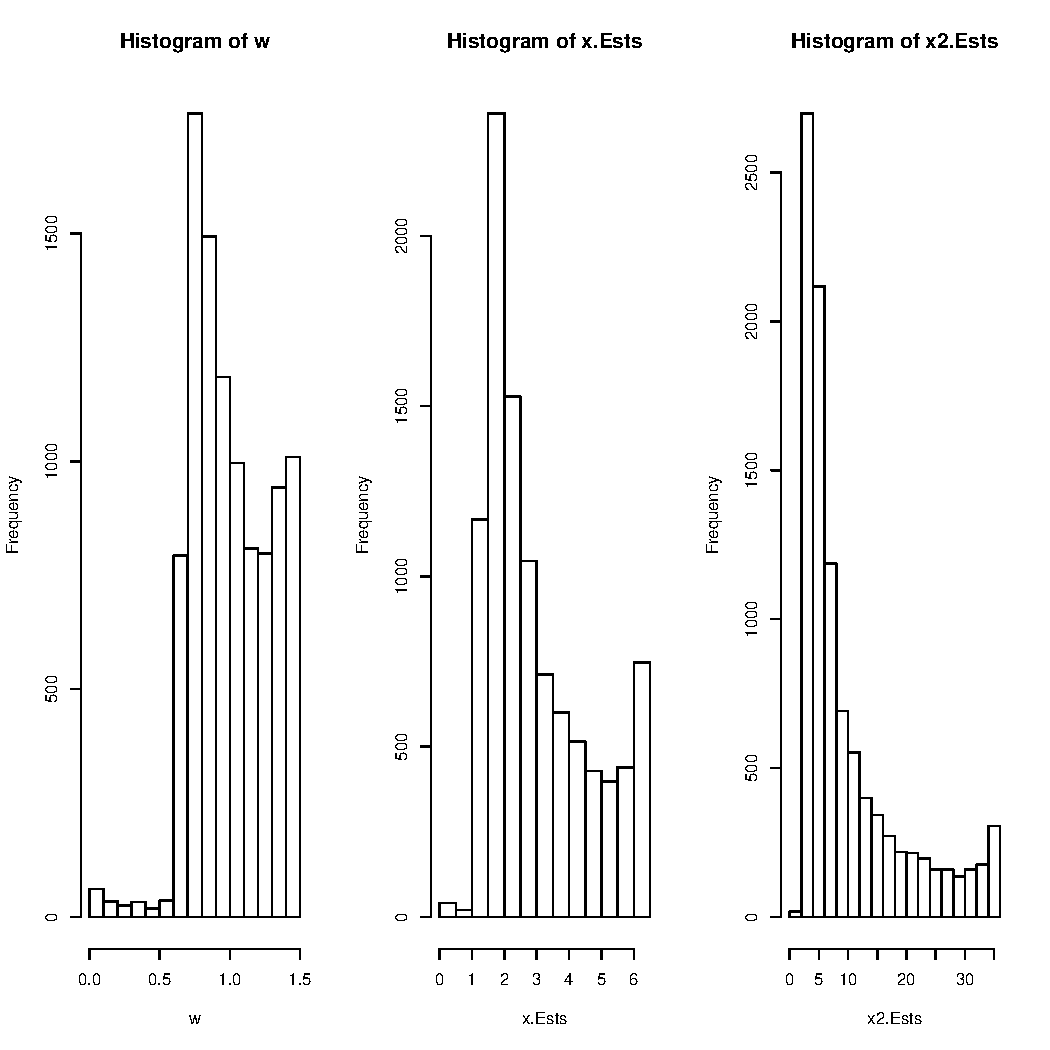
\includegraphics[width=\maxwidth]{figure/unnamed-chunk-2-1} 

\end{knitrout}
\subsection{Part (c)}
\begin{knitrout}
\definecolor{shadecolor}{rgb}{0.969, 0.969, 0.969}\color{fgcolor}\begin{kframe}
\begin{alltt}
\hlcom{################}
\hlcom{### Part (c) ###}
\hlcom{################}

\hlcom{#Proceeds in the same manner as Part (b)}
\hlcom{#only the functions are switched}
\hlkwd{set.seed}\hlstd{(}\hlnum{1}\hlstd{)}
\hlstd{m}  \hlkwb{<-} \hlnum{10000}
\hlstd{u} \hlkwb{<-} \hlkwd{runif}\hlstd{(m)}
\hlstd{smpls} \hlkwb{<-} \hlkwd{inverse.cdf.exp.shft}\hlstd{(u)}

\hlstd{f} \hlkwb{<-} \hlkwd{pareto}\hlstd{(smpls,} \hlkwc{alpha} \hlstd{= alpha,} \hlkwc{beta} \hlstd{= beta)}
\hlstd{g} \hlkwb{<-} \hlkwd{exp.shft}\hlstd{(smpls,} \hlkwc{lambda} \hlstd{= lambda,} \hlkwc{shft} \hlstd{= x.shft)}

\hlstd{w} \hlkwb{<-} \hlstd{f} \hlopt{/} \hlstd{g}

\hlstd{x.Ests}  \hlkwb{<-} \hlstd{smpls}\hlopt{*}\hlstd{w}
\hlstd{x2.Ests} \hlkwb{<-} \hlstd{smpls}\hlopt{^}\hlnum{2}\hlopt{*}\hlstd{w}

\hlkwd{print}\hlstd{(}\hlstr{"Estimate for Expectation Value of X is "}\hlstd{)}
\end{alltt}
\begin{verbatim}
## [1] "Estimate for Expectation Value of X is "
\end{verbatim}
\begin{alltt}
\hlkwd{print}\hlstd{(}\hlkwd{mean}\hlstd{(x.Ests))}
\end{alltt}
\begin{verbatim}
## [1] 2.903723
\end{verbatim}
\begin{alltt}
\hlkwd{print}\hlstd{(}\hlstr{"Estimate for Expectation Value of X^2 is "}\hlstd{)}
\end{alltt}
\begin{verbatim}
## [1] "Estimate for Expectation Value of X^2 is "
\end{verbatim}
\begin{alltt}
\hlkwd{print}\hlstd{(}\hlkwd{mean}\hlstd{(x2.Ests))}
\end{alltt}
\begin{verbatim}
## [1] 9.852741
\end{verbatim}
\begin{alltt}
\hlkwd{par}\hlstd{(}\hlkwc{mfrow}\hlstd{=}\hlkwd{c}\hlstd{(}\hlnum{1}\hlstd{,}\hlnum{3}\hlstd{))}
\hlcom{#histograms of weights, and values for expectation values of X and X^2}
\hlkwd{hist}\hlstd{(w)}
\hlkwd{hist}\hlstd{(x.Ests)}
\hlkwd{hist}\hlstd{(x2.Ests)}
\end{alltt}
\end{kframe}
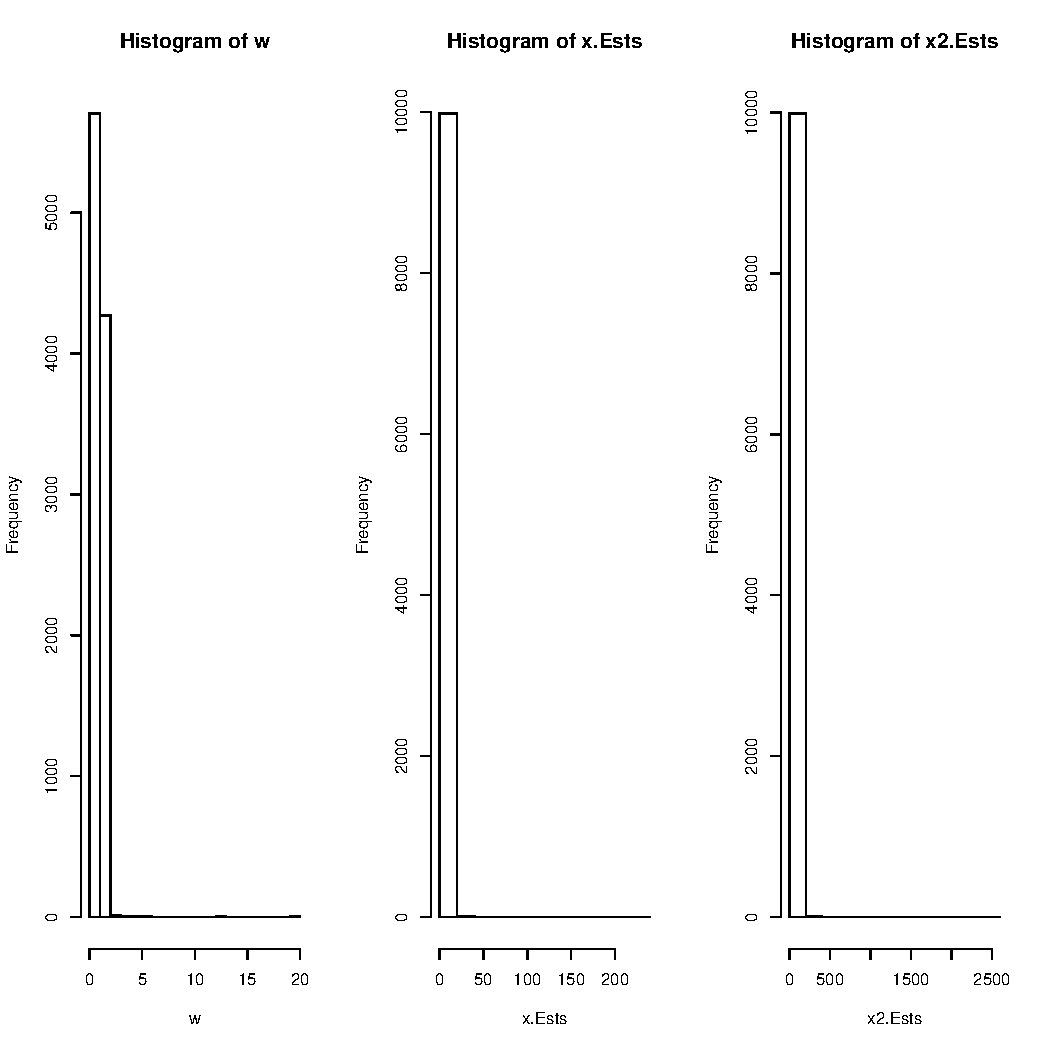
\includegraphics[width=\maxwidth]{figure/unnamed-chunk-3-1} 

\end{knitrout}
\section{Problem 2}
\begin{knitrout}
\definecolor{shadecolor}{rgb}{0.969, 0.969, 0.969}\color{fgcolor}\begin{kframe}
\begin{alltt}
\hlcom{##################}
\hlcom{### Question 2 ###}
\hlcom{##################}

\hlcom{### Taken from ps8.R provided by Chris ###}
\hlstd{theta} \hlkwb{<-} \hlkwa{function}\hlstd{(}\hlkwc{x1}\hlstd{,}\hlkwc{x2}\hlstd{)} \hlkwd{atan2}\hlstd{(x2, x1)}\hlopt{/}\hlstd{(}\hlnum{2}\hlopt{*}\hlstd{pi)}

\hlcom{#helical function}
\hlstd{f} \hlkwb{<-} \hlkwa{function}\hlstd{(}\hlkwc{x}\hlstd{) \{}
  \hlstd{f1} \hlkwb{<-} \hlnum{10}\hlopt{*}\hlstd{(x[}\hlnum{3}\hlstd{]} \hlopt{-} \hlnum{10}\hlopt{*}\hlkwd{theta}\hlstd{(x[}\hlnum{1}\hlstd{],x[}\hlnum{2}\hlstd{]))}
  \hlstd{f2} \hlkwb{<-} \hlnum{10}\hlopt{*}\hlstd{(}\hlkwd{sqrt}\hlstd{(x[}\hlnum{1}\hlstd{]}\hlopt{^}\hlnum{2} \hlopt{+} \hlstd{x[}\hlnum{2}\hlstd{]}\hlopt{^}\hlnum{2}\hlstd{)} \hlopt{-} \hlnum{1}\hlstd{)}
  \hlstd{f3} \hlkwb{<-} \hlstd{x[}\hlnum{3}\hlstd{]}
  \hlkwd{return}\hlstd{(f1}\hlopt{^}\hlnum{2} \hlopt{+} \hlstd{f2}\hlopt{^}\hlnum{2} \hlopt{+} \hlstd{f3}\hlopt{^}\hlnum{2}\hlstd{)}
\hlstd{\}}
\hlcom{### Taken from ps8.R provided by Chris ###}

\hlkwd{par}\hlstd{(}\hlkwc{mfrow}\hlstd{=}\hlkwd{c}\hlstd{(}\hlnum{3}\hlstd{,}\hlnum{3}\hlstd{))}
\hlcom{#Create perspective, contour, and image plots with constant z-conditions}
\hlcom{#scan over the values of x and y}
\hlcom{#[-100, 100] with step size = 1}
\hlcom{#hold z = -1, -5 and -10}
\hlkwa{for} \hlstd{(k} \hlkwa{in} \hlkwd{c}\hlstd{(}\hlnum{1}\hlstd{,}\hlnum{5}\hlstd{,}\hlnum{10}\hlstd{)) \{}
  \hlstd{x}\hlkwb{=}\hlkwd{seq}\hlstd{(}\hlopt{-}\hlnum{10}\hlstd{,}\hlnum{10}\hlstd{,}\hlnum{1}\hlstd{)}
  \hlstd{y}\hlkwb{=}\hlkwd{seq}\hlstd{(}\hlopt{-}\hlnum{10}\hlstd{,}\hlnum{10}\hlstd{,}\hlnum{1}\hlstd{)}
  \hlstd{x.len}\hlkwb{=} \hlkwd{length}\hlstd{(x)}
  \hlstd{y.len} \hlkwb{=} \hlkwd{length}\hlstd{(y)}
  \hlstd{z}\hlkwb{=}\hlkwd{array}\hlstd{(}\hlnum{0}\hlstd{,}\hlkwc{dim}\hlstd{=}\hlkwd{c}\hlstd{(x.len,y.len))}
  \hlcom{#scan over all values of x and y and hold z constant}
  \hlkwa{for} \hlstd{(i} \hlkwa{in} \hlnum{1}\hlopt{:}\hlstd{x.len)} \hlkwa{for} \hlstd{(j} \hlkwa{in} \hlnum{1}\hlopt{:}\hlstd{y.len) z[i,j]} \hlkwb{=} \hlkwd{f}\hlstd{(}\hlkwd{c}\hlstd{(x[i],y[j],}\hlopt{-}\hlstd{k))}
    \hlcom{#create plots -- perspective, contour, and image}
    \hlkwd{persp}\hlstd{(x, y, z,} \hlkwc{phi} \hlstd{=} \hlnum{20}\hlstd{,} \hlkwc{theta} \hlstd{=} \hlnum{40}\hlstd{)}
    \hlkwd{contour}\hlstd{(x, y, z)}
    \hlkwd{image}\hlstd{(x, y, z)}
\hlstd{\}}
\end{alltt}
\end{kframe}
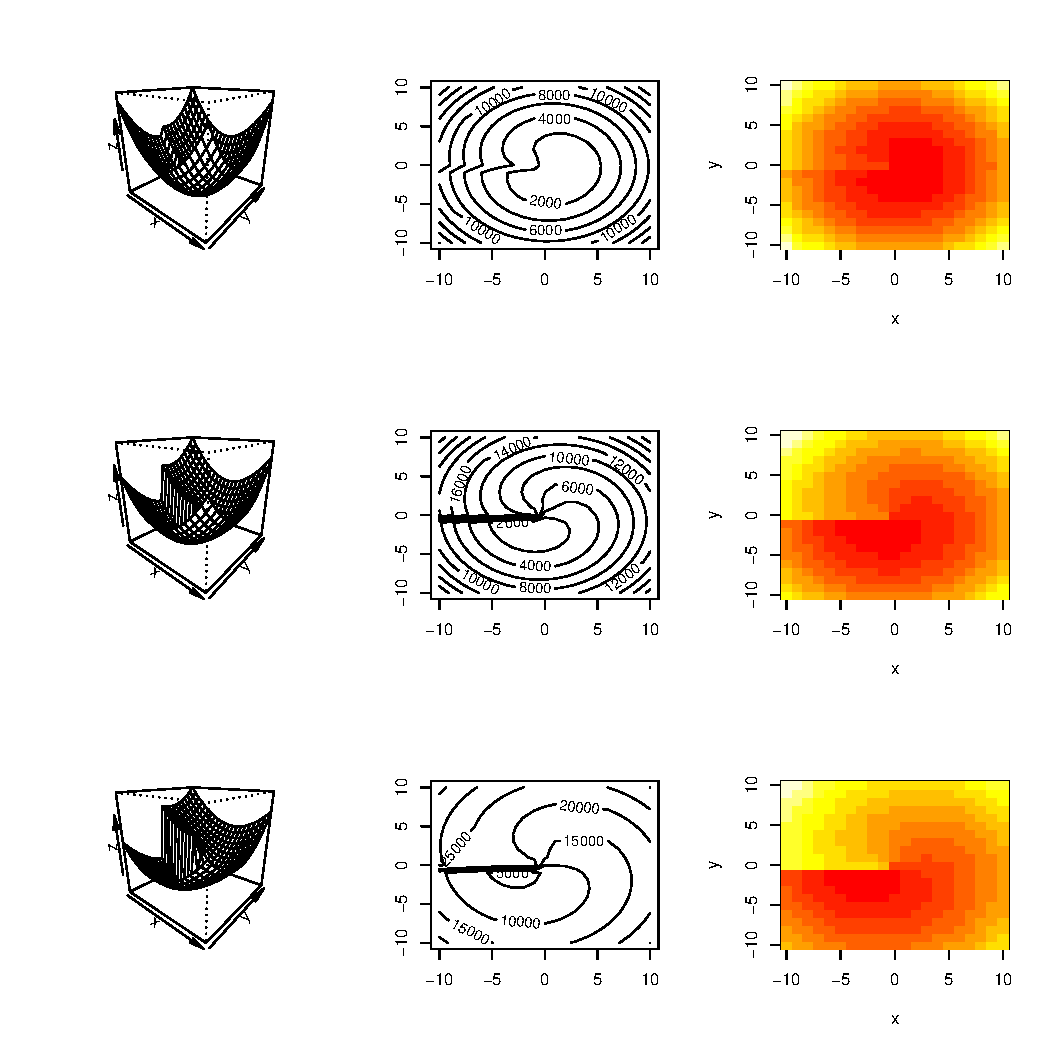
\includegraphics[width=\maxwidth]{figure/unnamed-chunk-4-1} 
\begin{kframe}\begin{alltt}
\hlcom{#Compare optimization methods for all values in x,y, and z ranges}
\hlcom{#[-100,100], step-size = 1}
\hlstd{x.seq} \hlkwb{<-} \hlkwd{seq}\hlstd{(}\hlopt{-}\hlnum{10}\hlstd{,}\hlnum{10}\hlstd{,}\hlnum{1}\hlstd{)}
\hlstd{y.seq} \hlkwb{<-} \hlkwd{seq}\hlstd{(}\hlopt{-}\hlnum{10}\hlstd{,}\hlnum{10}\hlstd{,}\hlnum{1}\hlstd{)}
\hlstd{z.seq} \hlkwb{<-} \hlkwd{seq}\hlstd{(}\hlopt{-}\hlnum{10}\hlstd{,}\hlnum{10}\hlstd{,}\hlnum{1}\hlstd{)}

\hlcom{#create empy vectors for optimization outputs}
\hlstd{optim.output} \hlkwb{<-} \hlkwd{c}\hlstd{()}
\hlstd{nlm.output}   \hlkwb{<-} \hlkwd{c}\hlstd{()}

\hlcom{#conducting optimization, scanning over all values}
\hlcom{#both optim and nlm studied}
\hlkwa{for} \hlstd{(i} \hlkwa{in} \hlstd{x.seq) \{}
  \hlkwa{for} \hlstd{(j} \hlkwa{in} \hlstd{y.seq) \{}
    \hlkwa{for} \hlstd{(k} \hlkwa{in} \hlstd{z.seq) \{}
      \hlstd{tmp.optim} \hlkwb{<-} \hlkwd{optim}\hlstd{(}\hlkwd{c}\hlstd{(i,j,k),} \hlkwc{fn} \hlstd{= f)}
      \hlstd{tmp.nlm}   \hlkwb{<-} \hlkwd{nlm}\hlstd{(}\hlkwc{p} \hlstd{=} \hlkwd{c}\hlstd{(i,j,k),} \hlkwc{f} \hlstd{= f)}
      \hlcom{#save outputs to initialized lists}
      \hlstd{optim.output} \hlkwb{<-}  \hlkwd{rbind}\hlstd{(optim.output,} \hlkwd{c}\hlstd{(tmp.optim}\hlopt{$}\hlstd{par, tmp.optim}\hlopt{$}\hlstd{value))}
      \hlstd{nlm.output}   \hlkwb{<-}  \hlkwd{rbind}\hlstd{(nlm.output,} \hlkwd{c}\hlstd{(tmp.nlm}\hlopt{$}\hlstd{estimate, tmp.nlm}\hlopt{$}\hlstd{minimum))}
    \hlstd{\}}
  \hlstd{\}}
\hlstd{\}}
\hlcom{#Print the resulting outputs from each optimization}
\hlkwd{head}\hlstd{(optim.output)}
\end{alltt}
\begin{verbatim}
##           [,1]          [,2]          [,3]         [,4]
## [1,] 1.0000192  0.0017768600  0.0035919425 7.132079e-05
## [2,] 0.9986558 -0.0008981530 -0.0018195403 1.989508e-04
## [3,] 1.0000462 -0.0063633215 -0.0099802284 1.021983e-04
## [4,] 0.9995174  0.0064526016  0.0096817711 1.501879e-04
## [5,] 1.0002442 -0.0014208359 -0.0027643164 3.900827e-05
## [6,] 0.9999825 -0.0004433395 -0.0008347427 2.394584e-06
\end{verbatim}
\begin{alltt}
\hlkwd{head}\hlstd{(nlm.output)}
\end{alltt}
\begin{verbatim}
##           [,1]          [,2]          [,3]         [,4]
## [1,] 1.0000000 -2.788850e-10 -4.093529e-10 4.726858e-19
## [2,] 1.0000000 -8.894507e-09 -7.034610e-09 5.131968e-15
## [3,] 1.0000000  1.858146e-09 -2.066969e-09 3.142904e-15
## [4,] 0.9999995 -8.223398e-05 -1.300839e-04 1.701008e-08
## [5,] 1.0000000 -5.687298e-11  1.608843e-10 1.285024e-17
## [6,] 1.0000000  1.206080e-09  1.864384e-09 1.203165e-17
\end{verbatim}
\begin{alltt}
\hlcom{#signifcant use of decimals make all answers unique}
\hlcom{#rounding to reduce this issue}
\hlcom{#rounding to two decimal places}
\hlcom{#printing unique results from rounded lists}

\hlkwd{head}\hlstd{(}\hlkwd{unique}\hlstd{(}\hlkwd{round}\hlstd{(optim.output,} \hlnum{2}\hlstd{)))}
\end{alltt}
\begin{verbatim}
##      [,1]  [,2]  [,3] [,4]
## [1,]    1  0.00  0.00    0
## [2,]    1 -0.01 -0.01    0
## [3,]    1  0.01  0.01    0
## [4,]    1  0.00  0.01    0
## [5,]    1  0.02  0.02    0
## [6,]    1  0.00 -0.01    0
\end{verbatim}
\begin{alltt}
\hlkwd{head}\hlstd{(}\hlkwd{unique}\hlstd{(}\hlkwd{round}\hlstd{(nlm.output,} \hlnum{2}\hlstd{)))}
\end{alltt}
\begin{verbatim}
##      [,1] [,2] [,3] [,4]
## [1,]    1    0    0    0
## [2,]   -8    0    5 4925
## [3,]   -7    0    5 3625
## [4,]   -6    0    5 2525
## [5,]   -5    0    5 1625
## [6,]   -5    0    6 1736
\end{verbatim}
\end{kframe}
\end{knitrout}
\section{Problem 3}
\subsection{Part (a)}
Mathematical derivation was done by hand and is attached to the hard-copy of this problem set.  Below is the pseudo-implementation of the EM algorithm for a censored linear regression.  In order to complete the math, I referenced the following article --
\newline
\newline
Park, Chanseok, Seong Beom, Lee. (2003). \emph{Parameter Estimation from Censored Samples using Expectation-Maximumization Algorithm}. Clemson University. https://arxiv.org/pdf/1203.3880.pdf.

\begin{knitrout}
\definecolor{shadecolor}{rgb}{0.969, 0.969, 0.969}\color{fgcolor}\begin{kframe}
\begin{alltt}
\hlcom{##################}
\hlcom{### Question 3 ###}
\hlcom{##################}

\hlcom{#cen.reg.EM <- name of EM algorithm}
\hlcom{#theta <- (b0, b1, s2) wher s2 = sigma^2}
\hlcom{#epsilon <- convergence condition tolerance}
\hlcom{#X <- xs needed for generation of slopes}
\hlcom{#Y <- Y_observed values}
\hlcom{#Z <- censored data values}
\hlcom{#tau <- censoring condition}


\hlstd{cen.reg.EM} \hlkwb{<-} \hlkwa{function}\hlstd{(}\hlkwc{theta}\hlstd{,} \hlkwc{epsilon}\hlstd{,} \hlkwc{X}\hlstd{,} \hlkwc{Y}\hlstd{,} \hlkwc{Z}\hlstd{,} \hlkwc{tau}\hlstd{) \{}
  \hlstd{t} \hlkwb{<-} \hlnum{0} \hlcom{#iterations counter}
  \hlstd{converge.cond} \hlkwb{<-} \hlnum{FALSE} \hlcom{#convergence initialization}

  \hlkwa{while}\hlstd{(}\hlopt{!}\hlstd{converge.cond) \{}
    \hlcom{#conduct calculations of theta(t+1)}
    \hlcom{#obtained by taking the derivatives of the}
    \hlcom{#log-likelihood of theta}
    \hlstd{prev.theta} \hlkwb{<-} \hlstd{theta}
    \hlcom{#tau star of truncated normal}
    \hlstd{tau1} \hlkwb{<-} \hlstd{(tau} \hlopt{-} \hlstd{(prev.theta[}\hlnum{2}\hlstd{]}\hlopt{+}\hlstd{prev.theta[}\hlnum{1}\hlstd{]}\hlopt{*}\hlstd{X)}\hlopt{/}\hlkwd{sqrt}\hlstd{(prev.theta[}\hlnum{3}\hlstd{]))}
    \hlcom{#length of data}
    \hlstd{n} \hlkwb{<-} \hlkwd{length}\hlstd{(X)}
    \hlcom{#position of truncation}
    \hlstd{c} \hlkwb{<-} \hlkwd{length}\hlstd{(Z)}
    \hlcom{#rho(tau1): rho of tau star (truncated normal)}
    \hlstd{rho} \hlkwb{<-} \hlkwd{dnorm}\hlstd{(tau1)} \hlopt{/} \hlstd{(}\hlnum{1} \hlopt{-} \hlkwd{pnorm}\hlstd{(tau1))}

    \hlstd{beta0.update} \hlkwb{<-} \hlstd{n}\hlopt{^-}\hlnum{1}\hlopt{*}\hlstd{(}\hlkwd{sum}\hlstd{(Z)} \hlopt{+} \hlstd{(n} \hlopt{-} \hlstd{c)}\hlopt{*}\hlstd{(prev.theta[}\hlnum{1}\hlstd{]} \hlopt{+} \hlstd{prev.theta[}\hlnum{2}\hlstd{]}\hlopt{*}\hlstd{X}
                                      \hlopt{+} \hlkwd{sum}\hlstd{(prev.theta[}\hlnum{3}\hlstd{]}\hlopt{*}\hlstd{rho)))}
    \hlstd{beta1.update} \hlkwb{<-} \hlstd{n}\hlopt{^-}\hlnum{1}\hlopt{*}\hlstd{(}\hlkwd{sum}\hlstd{(Z)} \hlopt{+} \hlstd{(n} \hlopt{-} \hlstd{c)}\hlopt{*}\hlstd{(prev.theta[}\hlnum{1}\hlstd{]} \hlopt{+} \hlstd{theta[}\hlnum{2}\hlstd{]}\hlopt{*}\hlstd{X}
                                      \hlopt{+} \hlkwd{sum}\hlstd{(prev.theta[}\hlnum{3}\hlstd{]}\hlopt{*}\hlstd{rho)))}
    \hlstd{sigma.update} \hlkwb{<-} \hlstd{n}\hlopt{^-}\hlnum{1}\hlopt{*}\hlstd{(}\hlkwd{sum}\hlstd{(Z}\hlopt{^}\hlnum{2}\hlstd{)} \hlopt{+} \hlstd{(n} \hlopt{-} \hlstd{c)}\hlopt{*}\hlstd{(prev.theta[}\hlnum{1}\hlstd{]} \hlopt{+} \hlstd{prev.theta[}\hlnum{2}\hlstd{]}\hlopt{*}\hlstd{X)}
                          \hlopt{*}\hlstd{((prev.theta[}\hlnum{1}\hlstd{]} \hlopt{+} \hlstd{prev.theta[}\hlnum{2}\hlstd{]}\hlopt{*}\hlstd{X)} \hlopt{+} \hlstd{prev.theta[}\hlnum{3}\hlstd{])} \hlopt{+}
                            \hlkwd{sum}\hlstd{((prev.theta[}\hlnum{1}\hlstd{]} \hlopt{+} \hlstd{prev.theta[}\hlnum{2}\hlstd{]}\hlopt{*}\hlstd{X} \hlopt{+} \hlstd{tau)}\hlopt{*}\hlkwd{sqrt}\hlstd{(prev.theta[}\hlnum{3}\hlstd{])}\hlopt{*}\hlstd{rho))}
                          \hlopt{+} \hlstd{(}\hlnum{1}\hlopt{/}\hlstd{n}\hlopt{^}\hlnum{2}\hlstd{)}\hlopt{*}\hlstd{(}\hlkwd{sum}\hlstd{(Z)} \hlopt{+} \hlstd{(n} \hlopt{-} \hlstd{c)}\hlopt{*}\hlstd{(prev.theta[}\hlnum{1}\hlstd{]} \hlopt{+} \hlstd{prev.theta[}\hlnum{2}\hlstd{]}\hlopt{*}\hlstd{X}
                          \hlopt{+} \hlkwd{sum}\hlstd{(prev.theta[}\hlnum{3}\hlstd{]}\hlopt{*}\hlstd{rho)))}
    \hlcom{#save to new theta}
    \hlstd{theta} \hlkwb{<-} \hlkwd{c}\hlstd{(beta0.update, beta1.update, sigma.update)}
    \hlstd{t} \hlkwb{<-} \hlstd{t} \hlopt{+} \hlnum{1} \hlcom{#iteration step}
    \hlcom{#Exit condition for the algorithm}
    \hlkwa{if}\hlstd{(}\hlkwd{max}\hlstd{(}\hlkwd{abs}\hlstd{(theta} \hlopt{-} \hlstd{prev.theta))} \hlopt{<} \hlstd{epsilon ) \{}
      \hlstd{converge.cond} \hlkwb{<-} \hlnum{TRUE}
    \hlstd{\}}
  \hlstd{\}}
  \hlcom{#return converged values and number of iterations}
  \hlkwd{return}\hlstd{(}\hlkwd{c}\hlstd{(theta, t))}

\hlstd{\}}
\end{alltt}
\end{kframe}
\end{knitrout}

\subsection{Part (b)}
For initialization conditions, I propose that the intercept, $\beta_0$, is set to zero, the slope, $\beta_1$, is set to 1, and the variance, $\sigma^2$, is set to 0.5.  This way, all of the values are on the same scale.
\subsection{Part (c)}
\subsection{Part (d)}
\end{document}
